%%
%% This is file `sample-sigplan.tex',
%% generated with the docstrip utility.
%%
%% The original source files were:
%%
%% samples.dtx  (with options: `sigplan')
%% 
%% IMPORTANT NOTICE:
%% 
%% For the copyright see the source file.
%% 
%% Any modified versions of this file must be renamed
%% with new filenames distinct from sample-sigplan.tex.
%% 
%% For distribution of the original source see the terms
%% for copying and modification in the file samples.dtx.
%% 
%% This generated file may be distributed as long as the
%% original source files, as listed above, are part of the
%% same distribution. (The sources need not necessarily be
%% in the same archive or directory.)
%%
%% The first command in your LaTeX source must be the \documentclass command.
\documentclass[sigplan,screen]{acmart}
\usepackage{algorithm}
\usepackage{algpseudocode}
%%
%% \BibTeX command to typeset BibTeX logo in the docs
\AtBeginDocument{%
  \providecommand\BibTeX{{%
    \normalfont B\kern-0.5em{\scshape i\kern-0.25em b}\kern-0.8em\TeX}}}

%% Rights management information.  This information is sent to you
%% when you complete the rights form.  These commands have SAMPLE
%% values in them; it is your responsibility as an author to replace
%% the commands and values with those provided to you when you
%% complete the rights form.
%%\setcopyright{acmcopyright}
%%\copyrightyear{2018}
%%\acmYear{2018}
%%\acmDOI{10.1145/1122445.1122456}

%% These commands are for a PROCEEDINGS abstract or paper.
\acmConference[Gwangju '21]{SEC@SAC '21: The Security Track at the ACM Symposium on Applied Computing}{March 22--26, 2021}{Gwangju, Korea}
%%\acmBooktitle{Woodstock '18: ACM Symposium on Neural Gaze Detection,
%%  June 03--05, 2018, Woodstock, NY}
%%\acmPrice{15.00}
%%\acmISBN{978-1-4503-XXXX-X/18/06}


%%
%% Submission ID.
%% Use this when submitting an article to a sponsored event. You'll
%% receive a unique submission ID from the organizers
%% of the event, and this ID should be used as the parameter to this command.
%%\acmSubmissionID{123-A56-BU3}

%%
%% The majority of ACM publications use numbered citations and
%% references.  The command \citestyle{authoryear} switches to the
%% "author year" style.
%%
%% If you are preparing content for an event
%% sponsored by ACM SIGGRAPH, you must use the "author year" style of
%% citations and references.
%% Uncommenting
%% the next command will enable that style.
%%\citestyle{acmauthoryear}

%%
%% end of the preamble, start of the body of the document source.
\begin{document}

%%
%% The "title" command has an optional parameter,
%% allowing the author to define a "short title" to be used in page headers.
\title{X-Pro: Distributed XDP Proxies against DDoS}

%%
%% The "author" command and its associated commands are used to define
%% the authors and their affiliations.
%% Of note is the shared affiliation of the first two authors, and the
%% "authornote" and "authornotemark" commands
%% used to denote shared contribution to the research.
\author{Syafiq Al Atiiq}
\email{syafiq_al.atiiq@eit.lth.se}
\affiliation{%
  \institution{LTH, Lund University}
  \city{Lund}
  \country{Sweden}
}
\author{Christian Gehrmann}
\email{christian.gehrmann@eit.lth.se}
\affiliation{%
  \institution{LTH, Lund University}
  \city{Lund}
  \country{Sweden}
}  

%%
%% The abstract is a short summary of the work to be presented in the
%% article.
\begin{abstract}
The concept of Internet of Things promised to connect billions of devices around the globe to the internet and capable to communicate each other. However, the device itself is especially vulnerable to be used as a bot to launch a massive Distributed-Denial-of-Service attack. The main problem with the IoT devices are usually resource-constrained, such that implementing a strong security protection is a non-trivial problem. Hence, they are easily turned from a usable embedded device into a bot for launching DDoS attack. 

A source-based DDoS detection could help reducing the impact of DDoS attack by blocking traffic from the source address of adversary. However, determining the legitimacy of the traffic close to the source is a hard problem, because the volume might not be big enough to be deemed as an attack. Also, from the economic standpoint, placing a classifier node close to the source is not incentivising the service provider. In this paper, we present a reverse-firewall proxy on the cloud working together as a distributed synchronous proxies to mitigate DDoS attack. The logic of the proxy is executed down to the kernel context, leveraging eXpress Data Path, a programmable network data path in the linux kernel. We evaluate the performance of our solution from several point of view. In conclusion, our solution offers a better decision making in terms of an attack traffic, as well as preserving the resource of the victims from a severe DDoS attack.  
\end{abstract}

%%
%% Keywords. The author(s) should pick words that accurately describe
%% the work being presented. Separate the keywords with commas.
\keywords{reverse-proxy, internet of things, denial of service, security}

%%
%% This command processes the author and affiliation and title
%% information and builds the first part of the formatted document.
\maketitle

\section{Introduction}
From September 2016, a tremendous distributed denial of service attack launched against several high-profile website on the internet, namely OVH \cite{ovh}, Dyn \cite{dyn}, and Krebs on Security \cite{kos}. Surprisingly, the source of the traffic came from a huge amount of the embedded devices turned into bots. These bots controlled by a master process, which later known as Mirai botnets \cite{203628}. The master process scanned the whole internet and infects embedded devices that still running with insecure default password. 

On the other hand, the emerging of Software Defined Networking (SDN) and Network Function Virtualization (NFV) bolster the shifting perspective of networking gears from a hardware oriented into a more "software based" product. This way, a system designer has more freedom on how they develop their networks, since most of the Network Functions (NF) can be installed into a white label hardware, i.e. standard commodity servers. Also, as the demand of the network capacity grows, the complexity of this "software based" network is also growing rapidly.

A software based network function also needs a fast packet processing function to achieve the same set of standard the hardware oriented networking gears already did. A normal packet processing procedure that rely on the user-space application in linux would be barely acceptable in terms of the performance. Therefore, a special purpose tool, namely Data Plane Development Kit (DPDK) \citep{dpdk}, solves this exact problem by entirely by-passing the operating system and let an application govern the network hardware directly. This comes at a price of dedicating a single (or more) CPU in the systems solely for packet processing function. Also, as the OS is by-passed, the application does not have the advantages of running many useful linux kernel module in the system.

An alternative to the previous solution is eXpress Data Path (XDP) \citep{10.1145/3281411.3281443}, where the fast packet processing is still achieved while keeping the operating system networking stack at the same time. The idea is to have an execution environment at the earliest possible point where packet can be tapped and apply a specific logic safely in the kernel context. 

In this paper, we introduce X-Pro, a well coordinated XDP proxies running together as a distributed systems to counteract DDoS, as we mentioned before about Mirai \cite{203628}. The detection happens at the earliest possible point, even before the packet touch the kernel in a white label hardware. The distributed proxies are sharing information between each other to assist in the decision making of packet filtering.  Different from prior source based DDoS mitigation techniques, our solution does not happen close to the source, i.e. embedded device, but rather at the cloud. This allows sharing of a real-time traffic situation for a very large number of devices at the proxy cloud side. This in turn gives much better possibilities to detect network based DDoS attempts as traffic information about DDoS attack destination targets is available to all proxies.

We have made a proof-of-concept implementation of X-Pro on a standard linux installation. As the proxy allows real-time information sharing in regards to the traffic condition, our protocol offers better ability to detect a possible DDoS attempt from a broader perspective. Our results show that the impact on the victim can be reduced significantly, even during a massive DDoS attack.

The rest of the paper is organized as follows. We discuss related works in Section II and background concepts in Section III. We provide the application scenario in Section IV. Section V presents scalable reverse firewall proxy, while in Section VI we provide a performance evaluation. Section VII draws our conclusions and anticipate future works.

\section{Related Work}
A major security problem in current networks is Distributed Denial-of-Service (DDoS) attacks where legitimate clients are used as bots. In particular, we consider the problem of source based DDoS in the context of internet of things network. It is considered as a non-trivial problem, since the source of the attacks can be distributed in different domains making it difficult for each of the source to detect and filter attack flows accurately. Also, it is difficult to differentiate between legitimate and attack traffic near the sources, since the volume of the traffic may not be big enough as the traffic typically aggregates at points closer to the destinations.

A conservative view of DDoS countermeasure procedure is mentioned by \cite{6489876}, in which there are two types of defense mechanisms, namely: (i) destination, and (ii). source based. Our work in this paper fell into the latter category. As we previously mentioned about SDN and NFV, there are also couple of proposals in securing the SDN based network from the DDoS attacks \cite{10.1145/3164541.3164562} \cite{10.1145/3360468.3368183}. JESS (Joint Entropy-based Security Scheme) \cite{8466805} proposed to enhance the SDN architecture against DDoS attacks by deploy a statistical solution. The model utilizes joint entropy to detect DDoS specific for SDN environment. 

Musumeci, et.al. \cite{9149043} took a step further by making a statement that SDN controllers might represent a critical point of failure for the whole network environment, especially when the controller are being attacked by DDoS. The proposed solution is to build a stateful data plane, in which the switches preserve a persistent memory of already processed packets. This memory is used to do attack detection with not so much involvement from the SDN controller.

The two previous SDN based DDoS detection are specific for the SDN network. A more general solution to DDoS countermeasure which has broader adoption in the current state-of-the-art networks is to use IP anycast \cite{rizvi2020anycast} \cite{10.1145/2987443.2987446}. By having a single IP anycast, the service provider is able to redistribute the traffic to a less crowded network in a case when DDoS attack is occured. This type of deployment is common in the current solution from DDoS protection provider, e.g. cloudflare \cite{anycast_cf}.

eXpress Data Path (XDP) \cite{10.1145/3281411.3281443} acts as an additional tool for DDoS countermeasure solutions by having a fast packet processor down in the kernel context. This would lead to a more efficient resource allocation, since there will be no memory allocation if the packet is not processed further and just dropped in the AF\_XDP. Instead of using a standalone XDP instance, we take a step further by building the synchronization function between XDP program running on each proxy through BPF maps communicated through a centralized database. The XDP logic can be loaded into a virtual network interface inside the VM. Furthermore, as our codebase does not require access to a specific kernel helper, X-Pro can be offloaded entirely to a smart-NIC \cite{8789414}.

As the informations on the state of the network are shared, proxy in different locations can catch-up the whole situation faster once DDoS happen in the network. This lead to a better DDoS mitigation in case the master of the botnets decide to launch the attack simultaniously using different bots from different locations. Lastly, since the detection of the legitimacy of the packets happens at the earliest possible point, even before reaching the kernel stack, the proxy does not have to allocate a lot of resource in handling the bogus messages. 

\section{Background}
\subsection{Express Data Path (XDP)}
Express Data Path (XDP) \cite{10.1145/3281411.3281443} is a novel programmable packet processing, living inside the kernel-space. XDP has been part of the mainland linux kernel since 4.8 \cite{xdp_kern}. One would argue that a kernel by-pass solution (i.e. DPDK \cite{dpdk}) would be more suitable for a fast packet processing. However, by-passing the kernel would neglect its rich features that might be useful for an intermediate node processing, i.e. firewall, router, proxy, etc. 

%\begin{figure}[htbp]
%\centerline{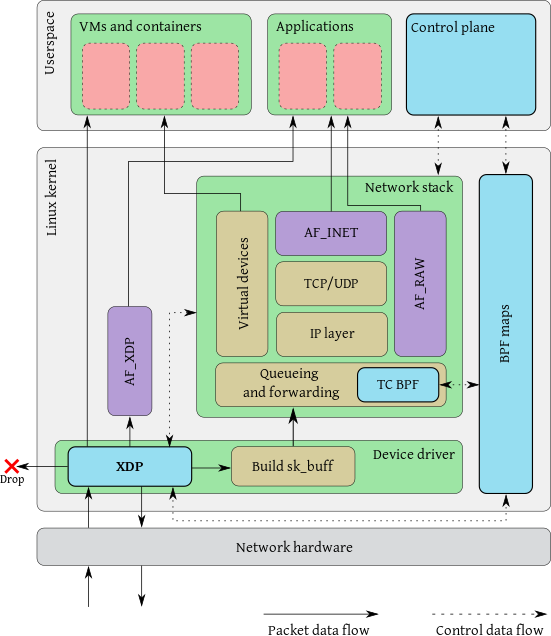
\includegraphics[scale=0.35]{pic/xdp-diagram-cut.png}}
%\caption{XDP Building Blocks \cite{10.1145/3281411.3281443}}
%\label{xdp}
%\end{figure}

When the packet arrives, the device driver runs and eBPF program within XDP hook. This process happens even before touching the packet data. During this early process, the eBPF program is able to determine the fate of the packet, in which one of the following would happen:
\begin{enumerate}
\item Drop the packet
\item Send the packet back out to the same interface
\item Redirect the packet, either to the same or different interface
\item Forward the packet to the userspace program, or
\item Allow the packet to be processed through a normal networking stack
\end{enumerate}
In accordance with that, our aim in this paper is to block the bogus packets at the earliest possible point, even before processed in the kernel. The process of selecting which packet is legitimate and/or which packet is bogus is communicated through multiple BPF maps. A more detailed description about how we utilize XDP is explained in the next chapter. 

The logic of eBPF program running inside XDP hook is written in high level language, i.e. C, and compiled into a bytecode. Kernel has the job to safeguard the eBPF program by verifying them. This verification happens during a load time of the program to the interface. If the code is safe, then the bytecode will be translated into a native machine instructions in order to achieve high performance.

\section{Reverse-Firewall-Proxy}
\subsection{Application Scenario}

\subsection{Proxy system architecture}
The proxy system consists of a set of proxies interconnected through an internal IP network. Each proxy is also assumed to have direct network connectivity. The proxy nodes shares filtering and also load information using a shared DB in the system. The solution is agnostic to a particular DB sharing method, but in our case, we use an in-memory database called Redis \cite{redis}. Our proxy architecture can be seen in the fig \ref{proxies}.

\begin{figure}[htbp]
\centerline{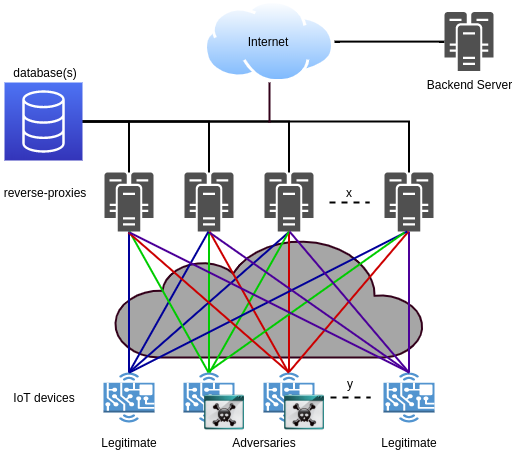
\includegraphics[scale=0.35]{pic/proxies.png}}
\caption{Mesh Network between IoT Devices and Reverse-Proxies}
\label{proxies}
\end{figure}

Each IoT unit must have the connectivity towards all available proxy, meaning that mesh network will be created between IoT units and the respective proxy. Also, as already mentioned previously, all proxies must have the same visibility in regards to which message needs to be blocked. Therefore, there has to be a mechanism to share information about this between proxies one way or another. 

As we would like to block the bogus messages at the earliest possible point, i.e. in the XDP hook, those information needs to be shared between kernel-space and user-space (and vice versa). This is where the BPF maps comes into place. As shown in figure \ref{proxies_xdp}, each proxy has a running redis instance, which syncronize each other through a process on each proxy, namely \textit{syncdb}. This process performs a synchronization protocol explained in subchapter \ref{psp}. The syncronized data then communicated to the eBPF program using another process called \textit{sync\_maps\_and\_ldb}. This process synchronize an already synched local redis instance with the BPF maps, which can be accessed directly by the eBPF program in the kernel.  

This way, we are able to pass the information between proxies without the need to send the invalid packet to the userspace. Hence, reducing the CPU utilization in the userland and allocate the CPU to a more important task, i.e. packet filtering in the kernel. Our argument is that the less tasks performed in the userspace, the more CPU can be utilized by the XDP to block the invalid messages, hence we get more packet filtering capacity in the kernel. Figure \ref{proxies_xdp} represent the connection between our packet filter mechanism with the syncronization function between databases.

\begin{figure}[htbp]
\centerline{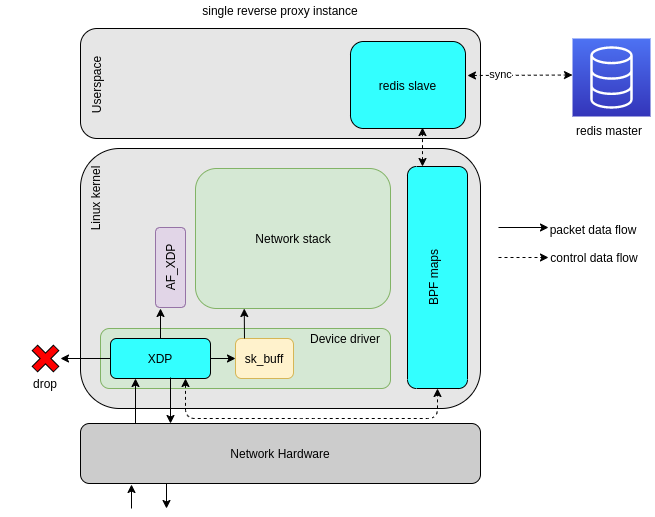
\includegraphics[scale=0.35]{pic/proxies_xdp.png}}
\caption{Syncronization between proxy and master DB}
\label{proxies_xdp}
\end{figure}

%\subsection{IoT unit architecture and general procedure}
%From the standpoint of IoT device, the proxy management is purely handled by the network interface or modems. This approach allows the modem to provide a standard network interface to the IoT OS. Figure \ref{iot_network} depict the relationship between IoT main MCU with the network interface. 

%\begin{figure}[htbp]
%\centerline{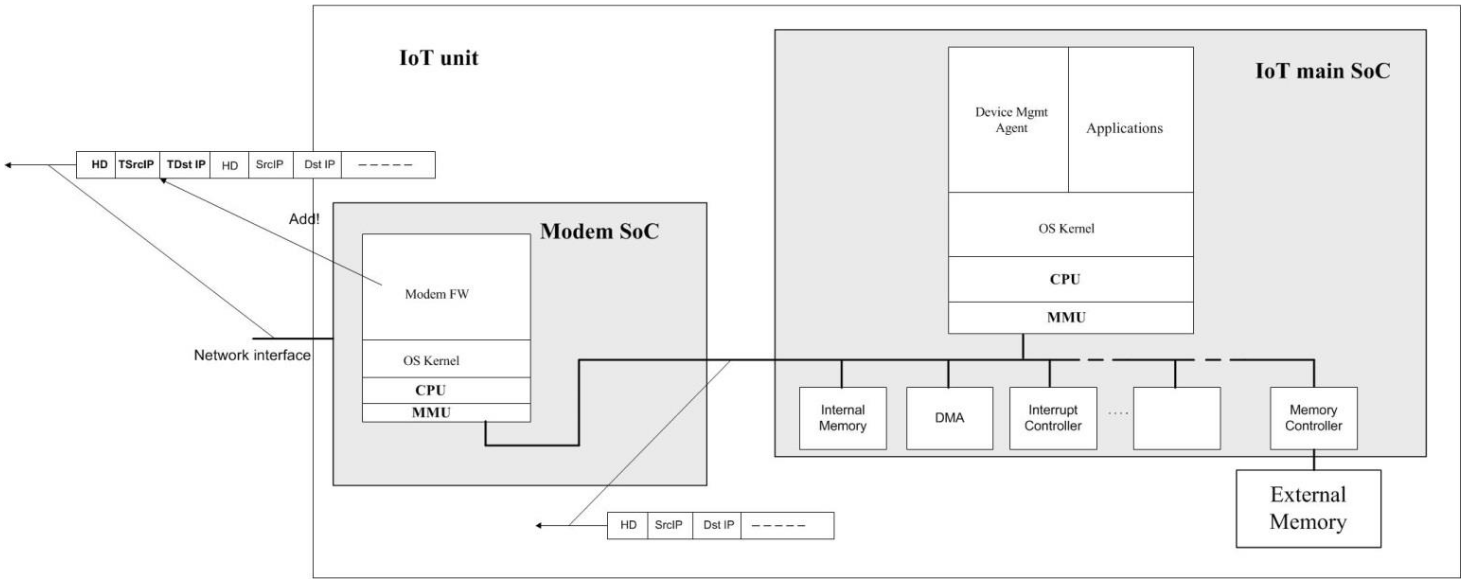
\includegraphics[scale=0.17]{pic/iot.png}}
%\caption{Dedicated Tunneled Network Interface (\textbf{a better and clearer picture will be created later})}
%\label{iot_network}
%\end{figure}

%The network modem is responsible for the proxy management for outbound traffic, i.e.:
%\begin{itemize}
%\item The network modem keeps track of available IoT proxies in the system and change “current destination proxy” if the one currently use is overloaded or unavailable. Information of availability and load is obtained through a separate proxy management protocol, explained in the next subchapter. 
%\item The modem tunnels all outbound traffic to the current proxy using either an IP tunnel, http or CoAP tunnel where the original source IP packet is encapsulated (not preventing IP or http level end-to-end security). Inbound traffic is treated completely transparently not affecting the modem or the IoT system at all.
%\end{itemize}

\section{Algorithm}
\subsection{Notations}
\begin{itemize}
\item Set of client devices in the system: $U$
\item An client device: $u \in U$
\item Set of proxies devices in the system: $P$
\item Proxy: $p \in P$
\item A unique index given to a client: $i$
\item An client device with index i: $u_i$
\item A proxy unique network address associated with a proxy: $j$
\item A proxy with address j: $p_j$
\item Work load of a proxy unit: $W$
\item Work load threshold of a proxy unit: $T_W$
\item Time stamp indicating the "oldest time" packet time for a particular $(i,D_{addr})$ pair: $ts_1$
\item Time stamp indicating the "most recent" packet time for a particular $(i,D_{addr})$ pair: $ts_2$
\item Packet counter or a particular $(i,D_{addr})$ pair: $c$
\item Delta packet counter (internally within a proxy) counter for a particular $(i,D_{addr})$ pair: $dc$
\item First filtering reset threshold used by a proxy: $T_{T1}$
\item Filtering minimum measure time threshold used by a proxy: $T_{T2}$
\item Second filtering minimum measure time threshold used by a proxy: $T_{T3}$
\item Fourth filtering minimum measure time threshold used by a proxy: $T_{T4}$
\item First packet maximum allowed frequency threshold used by a proxy: $T_{F1}$
\item Second packet maximum allowed frequency threshold used by a proxy: $T_{F2}$
\item Frequency division factor: $r^2$
\item Destination IP address of a packet: $D_{addr}$
\end{itemize}

\subsection{Proxy Synchronization Protocol}
\label{psp}
In order to have the same visibility on every proxy, one needs to have a synchronization function between them. This section explain in more detail those function, which has been implemented in our proof of concept inside the \textit{syncdb} process. 

For every time period $t$, each proxy $p_j$ performs the synchronization procedure with the master database, described in the algorithm \ref{alg_psp}. The initial process started with $p_j$ updates its current workload to the $M_{DB}$, which then replied by $M_{DB}$ with the information containing the workload for all other proxies except $p_j$. $p_j$ iterate through every $(i, D_{addr})$ inside the $M_{DB}$, and for each pair of $(i, D_{addr})$, $p_j$ looks up at the local database $L_{DB}$. If $L_{DB}$ contains information about $(i, D_{addr})$, it checks whether $mark$ is equal to 1, together with if $ts_1'$ minus $ts_1$ is greater than $T_{T1}$. If both conditions hold, both local value of $mark'$ and $dc'$ is set to 0, and the value of $ts_1$, $ts_2$ and $c$ is updated from the local value in $p_j$.

On the other hand, if both conditions do not hold, $mark'$ is set to 0. If local value $ts_2'$ is less than $M_{DB}$'s value $ts_2$, the local value is updated with the remote master database value. Furthermore, if $ts_2'$ minus $ts_1$ is greater than the fourth filtering minimum measure time threshold used by a proxy, $T_{T4}$, then the local value of $ts_1'$ is updated through the following equation : $ts_2'-(ts_2'-ts_1)/r$. The rest of the process is described in the algorithm \ref{alg_psp}. 

\begin{algorithm}
\caption{Proxy Synchronization Protocol}
\label{alg_psp}
\begin{algorithmic}[1]
\State $p_j$ send the $W$ value to $M_{DB}$
\State $p_j$ reads the current workload for all other proxies in the system, $\{W_k\}, p_k \in P, k \neq i$
\State $p_j$ looks all the pair $(i, D_{addr})$, for $u_i \in U$
\For{each $(i, D_{addr})$ in $M_{DB}$}
	\If{$L_{DB} \ni i, D_{addr}$}
		\If {$(mark' = 1$ and $ts_1' - ts_1 > T_{T1})$} 
			\State $<mark' = 0, dc' = 0>$
			\State $<ts_1=ts_1', ts_2=ts_2', c=c'>$
		\Else
			\State $<mark' = 0>$
			\If{$ts_2'<ts_2$}
				\State $<ts_2'=ts_2>$
			\ElsIf{$ts_2'-ts_1>T_{T4}$}
				\State $<ts_1'=ts_2'-(ts_2'-ts_1)/r>$
				\State $<c = \lfloor c/r \rfloor, ts_1=ts_1', ts_2=ts_2'>$
			\Else
				\State $<ts_2=ts_2'>$
			\EndIf
			
			\If{$ts_1'>ts_1$}
				\State $<ts_1'=ts_1>$
			\ElsIf{$ts_2'-ts_1'>T_{T4}$}
				\State $<ts_1=ts_1'>$
			\EndIf
			\State $<c'=c+dc', c=c', dc'=0>$
		\EndIf
	\Else
		\State $<ts_1'=ts_1, ts_2'=ts_2>$
		\State $<c'=c, dc'= 0, mark'=0>$
	\EndIf
\EndFor
\For{each $(i, D_{addr})$ in $L_{DB}$}
	\If{$M_{DB} \nni i, D_{addr}$}
		\State $<ts_1=ts_1', ts_2=ts_2', c=c'>$
	\EndIf
\EndFor
\end{algorithmic}
\end{algorithm}

\subsection{Packet Filtering Procedures}
When the packet arrives at the proxy, the procedures described in the algorithm \ref{alg_pfs} takes place. All the process in this part, happens inside the kernel space, within the $xdp\_prog\_kern$ mentioned in the figure \ref{proxies_xdp}. Therefore, the local database $L_{DB}$ we mention in this section means a bpf map, not a redis instance.

Initially, $p_j$ looks up and read the time stamps $ts_1'$ and $ts_2'$ for the record $(i, D_{addr})$ from the local database $L_{DB}$. If the record is found, $p_j$ compares the difference between the current time and $ts_2'$ with the first filtering reset threshold $T_{T1}$. If the difference value is bigger than $T_{T1}$, then $ts_1'$ is set to be the current time, $c'$ and $dc$ are reset to be 0 and $mark$ equal to 1. 

On the other hand, if $L_{DB}$ does not contain $(i, D_{addr})$, both $ts_1'$ and $ts_2'$ will be set to the current time, as well as resetting $c', dc$ and $mark$ to 0. The next step is to increase both the counter $c'$ and the counter difference $dc$ values with 1, and set $ts_2'$ with the current time. 

If the difference between $ts_2'$ and $ts_1'$ is larger than the second filtering minimum measure time threshold $T_{T2}$, then $p_j$ compares the value of $c'$ divided by the difference of $ts_1'$ and $ts_2'$ with the first packet maximum allowed frequency threshold, $T_{F1}$. If its greater than $T_{F1}$, the respective packet is dropped by the XDP, followed by sending an overload warning to the responsible administrator. 

If the packet passed through the previous checks, further packet processing involving statistical measurement is performed. First, $p_j$ calculates the minimum value of $ts_1$ corresponding to the same $D_{addr}$ from all the set of $U$, namely $ts_1*$. Second, it calculates the maximum value of $ts_2$ and the sum of $c+dc$ from the same set $U$, namely $ts_2*$ and $c*$ respectively. If $c*$ divided by $ts_2*$ minus $ts_1*$ is greater than $T_{F2}$, the respective packet $(i, D_{addr})$ is dropped, otherwise the packet is forwarded to $D_{addr}$.

\begin{algorithm}
\caption{Packet Filtering Procedures}
\label{alg_pfs}
\begin{algorithmic}[1]
\State $<$Lookup $ts_1', ts_2',c$ for record $(i,D_{addr})$ in $L_{DB}>$
\If{record found}
	\If{$t-ts_2'>T_{T1}$}
		\State $ts_1'=t,c'=0,dc=0,mark=1$
	\Else
		\State $<$do nothing$>$
	\EndIf
\Else
\State $ts_1'=ts_2'=t, c'=0, dc=0, mark=0$
\EndIf
\State $c'=c'+1, dc=dc+1, ts_2'=t$
\If{$ts_2'-ts_1'>T_{T2}$}
	\If{$c'/(ts_2'-ts_1') > T_{F1}$}
		\State $<$Drop packet$>$
		\State $<$Send an overload warning$>$
	\EndIf
\EndIf
\State $ts_1* = \min_{u_i \in U_{D_{addr}}} {ts_1}_i'$
\State $ts_2* = \max_{u_i \in U_{D_{addr}}} {ts_2}_i'$
\State $c* = \Sigma_{u_i \in U_{D_{addr}}} (c_i+dc_i)$
\If{$ts_2*-ts_1*>T_{T3}$}
	\If{$c*/(ts_2*-ts_1*)>T_{F2}$}
		\State $<$Drop packet$>$
	\EndIf
\EndIf
\State $<$forward packet$>$
\end{algorithmic}
\end{algorithm}

\section{Experimental Evaluation}
To evaluate X-Pro, we have developed a proof of concept of the implementation. Both the proxies and the centralized database are implemented as a virtual machine on Fedora 30 operating system, running kernel version 5.6. Our implementation is as an open-source software at \cite{xpro}. This section discusses the results from our experimental evaluation, following different scenarios in the proxy side. We show that, by placing the logic of distributed proxy at the earliest possible point, even before reaching the kernel, we can have a decent performance of dropping undesired packets. 

Our experiment follows the scenario in figure \ref{proxies}, deployed over a local ethernet network. All of the VMs of the proxies and centralized database are running with one vCPU and 1024 MB of memory. 

\subsection{Results}

\section{Conclusion and Future Work}

\bibliographystyle{ACM-Reference-Format}
\bibliography{krep}

\end{document}
\endinput